\section{Memory Alignment}

\frame{\tableofcontents[currentsection]}

\begin{frame}
  \frametitle{Reading from RAM}
  \begin{itemize}
    \item RAM is not organised as a series of bytes
    \item RAM is organised as a series of chunks
          \begin{itemize}
            \item For example, chunk of $4$ bytes long
          \end{itemize}
    \item Reading from RAM = reading one complete chunk
  \end{itemize}
  \begin{center}
    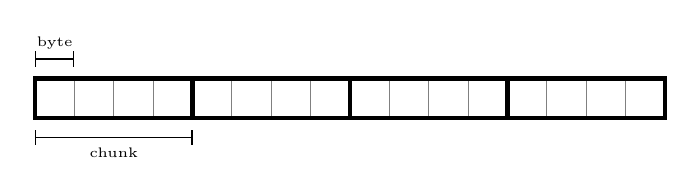
\begin{tikzpicture}
      \draw[thin,gray] (0,0) grid[xstep=0.5cm,ystep=0.5cm] (8,0.5);
      \draw[ultra thick] (0,0) grid[xstep=2cm,ystep=0.5cm] (8,0.5);
      \draw[ultra thick] (0,0) rectangle (8,0.5);

      \draw[|-|] (0,0.75) -- ++(0.5,0) node[midway,above,font=\tiny] {byte};
      \draw[|-|] (0,-0.25) -- ++(2,0) node[midway,below,font=\tiny] {chunk};
    \end{tikzpicture}
  \end{center}
\end{frame}

\begin{frame}
  \frametitle{Reading Aligned Block from RAM}
  \begin{center} \ttfamily\Large
    MOV EAX, [ESI]
  \end{center}
  \begin{center}
    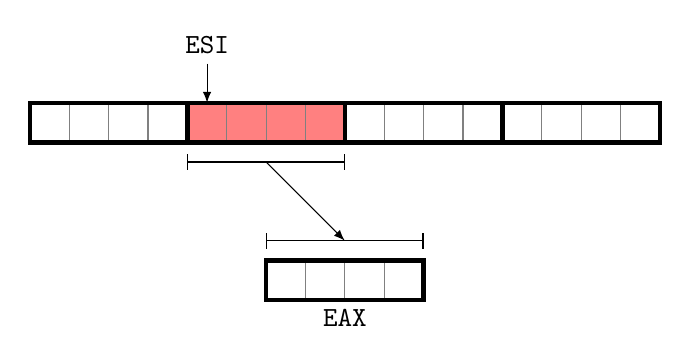
\begin{tikzpicture}
      \draw[fill=red!50] (2,0) rectangle ++(2,0.5);

      \draw[thin,gray] (0,0) grid[xstep=0.5cm,ystep=0.5cm] (8,0.5);
      \draw[ultra thick] (0,0) grid[xstep=2cm,ystep=0.5cm] (8,0.5);
      \draw[ultra thick] (0,0) rectangle (8,0.5);

      \draw[-latex] (2.25,1) -- ++(0,-0.5) node[above,at start,font=\ttfamily] {ESI};

      \draw[thin,gray] (3,-2) grid[xstep=0.5cm,ystep=0.5cm] ++(2,0.5);
      \draw[ultra thick] (3,-2) rectangle ++(2,0.5);

      \node[anchor=north,font=\ttfamily] at (4,-2) {EAX};

      \draw[|-|] (2,-0.25) -- ++(2,0);
      \draw[|-|] (3,-1.25) -- ++(2,0);
      \draw[-latex] (3,-0.25) -- (4,-1.25);
    \end{tikzpicture}
  \end{center}
  \begin{center}
    Reading a chunk from RAM to register happens in one step
  \end{center}
\end{frame}

\begin{frame}
  \frametitle{Reading Unaligned Block from RAM}
  \begin{center}
    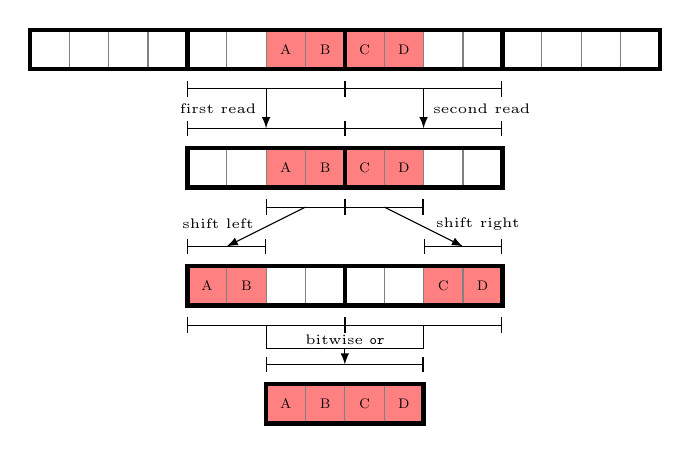
\begin{tikzpicture}[label/.style={font=\scshape\tiny}]
      \draw[fill=red!50] (3,0) rectangle ++(2,0.5);
      \draw[fill=red!50] (3,-1.5) rectangle ++(2,0.5);
      \draw[fill=red!50] (2,-3) rectangle ++(1,0.5);
      \draw[fill=red!50] (5,-3) rectangle ++(1,0.5);
      \draw[fill=red!50] (3,-4.5) rectangle ++(2,0.5);

      \draw[thin,gray] (0,0) grid[xstep=0.5cm,ystep=0.5cm] (8,0.5);
      \draw[ultra thick] (0,0) grid[xstep=2cm,ystep=0.5cm] (8,0.5);
      \draw[ultra thick] (0,0) rectangle (8,0.5);

      \draw[thin,gray] (2,-1.5) grid[xstep=0.5cm,ystep=0.5cm] ++(4,0.5);
      \draw[ultra thick] (2,-1.5) grid[xstep=2cm,ystep=0.5cm] ++(4,0.5);
      \draw[ultra thick] (2,-1.5) rectangle ++(4,0.5);

      \draw[thin,gray] (2,-3) grid[xstep=0.5cm,ystep=0.5cm] ++(4,0.5);
      \draw[ultra thick] (2,-3) grid[xstep=2cm,ystep=0.5cm] ++(4,0.5);
      \draw[ultra thick] (2,-3) rectangle ++(4,0.5);

      \draw[thin,gray] (3,-4.5) grid[xstep=0.5cm,ystep=0.5cm] ++(2,0.5);
      \draw[ultra thick] (3,-4.5) rectangle ++(2,0.5);

      \draw[|-|] (2,-0.25) -- ++(2,0);
      \draw[|-|] (2,-0.75) -- ++(2,0);
      \draw[-latex] (3,-0.25) -- (3,-0.75) node[left,font=\tiny,midway] {first read};

      \draw[|-|] (4,-0.25) -- ++(2,0);
      \draw[|-|] (4,-0.75) -- ++(2,0);
      \draw[-latex] (5,-0.25) -- (5,-0.75) node[right,font=\tiny,midway] {second read};

      \draw[|-|] (3,-1.75) -- ++(1,0);
      \draw[|-|] (2,-2.25) -- ++(1,0);
      \draw[-latex] (3.5,-1.75) -- (2.5,-2.25) node[left,font=\tiny,midway,xshift=-1pt,yshift=1pt] {shift left};

      \draw[|-|] (4,-1.75) -- ++(1,0);
      \draw[|-|] (5,-2.25) -- ++(1,0);
      \draw[-latex] (4.5,-1.75) -- (5.5,-2.25) node[right,font=\tiny,midway,xshift=1pt,yshift=1pt] {shift right};

      \draw[|-|] (2,-3.25) -- ++(2,0);
      \draw[|-|] (4,-3.25) -- ++(2,0);
      \draw[|-|] (3,-3.75) -- ++(2,0);
      \draw[-latex] (3,-3.25) -- ++(0,-0.3) -- ++(1,0) -- ++(0,-0.2);
      \draw (5,-3.25) -- ++(0,-0.3) -- ++(-1,0);
      \node[font=\tiny,anchor=south] at (4,-3.625) {bitwise \texttt{or}};

      \node[label] at (3.25,0.25) {A};
      \node[label] at (3.75,0.25) {B};
      \node[label] at (4.25,0.25) {C};
      \node[label] at (4.75,0.25) {D};

      \node[label] at (3.25,-1.25) {A};
      \node[label] at (3.75,-1.25) {B};
      \node[label] at (4.25,-1.25) {C};
      \node[label] at (4.75,-1.25) {D};

      \node[label] at (2.25,-2.75) {A};
      \node[label] at (2.75,-2.75) {B};
      \node[label] at (5.25,-2.75) {C};
      \node[label] at (5.75,-2.75) {D};

      \node[label] at (3.25,-4.25) {A};
      \node[label] at (3.75,-4.25) {B};
      \node[label] at (4.25,-4.25) {C};
      \node[label] at (4.75,-4.25) {D};
    \end{tikzpicture}
  \end{center}
  \begin{center}
    Reading 4 bytes that do not correspond to a chunk (i.e.~nonaligned) takes many steps
  \end{center}
\end{frame}

\begin{frame}
  \frametitle{Unaligned Memory Reads}
  \begin{itemize}
    \item If the word you need to read does not fit in one chunk, multiple reads will be necessary
    \item General rule of thumb: align $2^N$ sized words on a $2^N$-divisible memory address
          \begin{itemize}
            \item \texttt{uint8\_t} (1 byte long) can start anywhere
            \item \texttt{uint16\_t} (2 bytes) should start on address divisible by 2
            \item \texttt{uint32\_t} should start on address divisible by 4
            \item \texttt{uint64\_t} should start on address divisible by 8
          \end{itemize}
    \item This is generally done automatically by the compiler
  \end{itemize}
\end{frame}

\begin{frame}
  \frametitle{Size of Data Structures}
  \code[language=c++14]{sizeof.cpp}
  \begin{itemize}
    \item Should be $1+4+1+4 = 10$ bytes large
    \item \texttt{sizeof(Foo)} returns \texttt{16}
    \item Compiler leaves ``gaps'' so as to align \texttt{b} and \texttt{d} correctly
  \end{itemize}
\end{frame}

\begin{frame}
  \frametitle{\texttt{Foo} Memory Layout}
  \structure{Without Memory Alignment}
  \begin{center}
    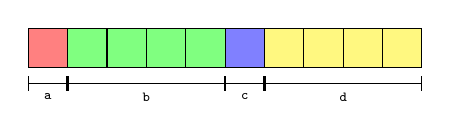
\begin{tikzpicture}
      \draw[fill=red!50] (0,0) rectangle ++(0.5,0.5);
      \draw[fill=green!50] (0.5,0) rectangle ++(2,0.5);
      \draw[fill=blue!50] (2.5,0) rectangle ++(0.5,0.5);
      \draw[fill=yellow!50] (3,0) rectangle ++(2,0.5);
      \draw[thin] (0,0) grid[xstep=0.5cm,ystep=0.5cm] ++(5,0.5);
     
      \begin{scope}[yshift=-2mm]
        \draw[|-|] (0,0) -- ++(0.5,0) node[midway,below,font=\tiny\ttfamily] {a};
        \draw[|-|] (0.5,0) -- ++(2,0) node[midway,below,font=\tiny\ttfamily] {b};
        \draw[|-|] (2.5,0) -- ++(0.5,0) node[midway,below,font=\tiny\ttfamily] {c};
        \draw[|-|] (3,0) -- ++(2,0) node[midway,below,font=\tiny\ttfamily] {d};
      \end{scope}
    \end{tikzpicture}
  \end{center}
  \structure{With Memory Alignment}
  \begin{center}
    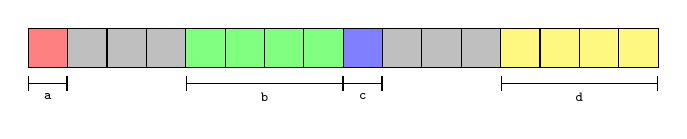
\begin{tikzpicture}
      \draw[fill=gray!50] (0,0) rectangle ++(8,0.5);
      \draw[fill=red!50] (0,0) rectangle ++(0.5,0.5);
      \draw[fill=green!50] (2,0) rectangle ++(2,0.5);
      \draw[fill=blue!50] (4,0) rectangle ++(0.5,0.5);
      \draw[fill=yellow!50] (6,0) rectangle ++(2,0.5);
      \draw[thin] (0,0) grid[xstep=0.5cm,ystep=0.5cm] ++(8,0.5);

      \begin{scope}[yshift=-2mm]
        \draw[|-|] (0,0) -- ++(0.5,0) node[midway,below,font=\tiny\ttfamily] {a};
        \draw[|-|] (2,0) -- ++(2,0) node[midway,below,font=\tiny\ttfamily] {b};
        \draw[|-|] (4,0) -- ++(0.5,0) node[midway,below,font=\tiny\ttfamily] {c};
        \draw[|-|] (6,0) -- ++(2,0) node[midway,below,font=\tiny\ttfamily] {d};
      \end{scope}
    \end{tikzpicture}
  \end{center}
  \begin{itemize}
    \item Grey: unused memory
    \item It would be better to rearrange members
          \begin{itemize}
            \item \texttt{a, c, b, d} would be optimal
            \item Compiler will always preserve order
            \item You need to rearrange yourself
          \end{itemize}
  \end{itemize}
\end{frame}

\begin{frame}
  \frametitle{Arrays}
  \begin{itemize}
    \item Extra complication: arrays
    \item We focused on aligning the members of one object
    \item What if we consider an array of such objects?
  \end{itemize}
\end{frame}

\begin{frame}
  \frametitle{Arrays}
  \code[language=c++14,font=\small,width=.5\linewidth]{int-char.cpp}
  \begin{center}
    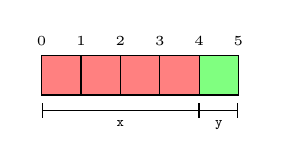
\begin{tikzpicture}
      \draw[fill=red!50] (0,0) rectangle ++(2,0.5);
      \draw[fill=green!50] (2,0) rectangle ++(0.5,0.5);
      \draw[thin] (0,0) grid[xstep=0.5cm,ystep=0.5cm] ++(2.5,0.5);

      \foreach[evaluate={\i*0.5} as \x] \i in {0,...,5} {
        \node[font=\tiny,anchor=south] at (\x,0.5) {\i};
      }

      \begin{scope}[yshift=-2mm]
        \draw[|-|] (0,0) -- ++(2,0) node[midway,below,font=\tiny\ttfamily] {x};
        \draw[|-|] (2,0) -- ++(0.5,0) node[midway,below,font=\tiny\ttfamily] {y};
      \end{scope}
    \end{tikzpicture}
  \end{center}
  \begin{itemize}
    \item Seems ok
    \item \texttt{x} is 4 bytes long and starts at 0
    \item \texttt{y} is 1 byte long, can start anywhere
    \item Members are aligned
  \end{itemize}
\end{frame}

\begin{frame}
  \frametitle{Arrays}
  \code[language=c++14,font=\small,width=.5\linewidth]{int-char.cpp}
  \begin{center}
    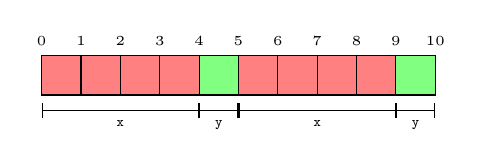
\begin{tikzpicture}
      \draw[fill=red!50] (0,0) rectangle ++(2,0.5);
      \draw[fill=green!50] (2,0) rectangle ++(0.5,0.5);
      \draw[fill=red!50] (2.5,0) rectangle ++(2,0.5);
      \draw[fill=green!50] (4.5,0) rectangle ++(0.5,0.5);
      \draw[thin] (0,0) grid[xstep=0.5cm,ystep=0.5cm] ++(5,0.5);

      \foreach[evaluate={\i*0.5} as \x] \i in {0,...,10} {
        \node[font=\tiny,anchor=south] at (\x,0.5) {\i};
      }

      \begin{scope}[yshift=-2mm]
        \draw[|-|] (0,0) -- ++(2,0) node[midway,below,font=\tiny\ttfamily] {x};
        \draw[|-|] (2,0) -- ++(0.5,0) node[midway,below,font=\tiny\ttfamily] {y};
        \draw[|-|] (2.5,0) -- ++(2,0) node[midway,below,font=\tiny\ttfamily] {x};
        \draw[|-|] (4.5,0) -- ++(0.5,0) node[midway,below,font=\tiny\ttfamily] {y};
      \end{scope}
    \end{tikzpicture}
  \end{center}
  \begin{itemize}
    \item Array of 2 \texttt{foo}s
    \item Second \texttt{foo}'s \texttt{x} starts at address \texttt{5}
    \item I.e.~it is not aligned correctly
  \end{itemize}
\end{frame}

\begin{frame}
  \frametitle{Arrays}
  \begin{itemize}
    \item To ensure that all members are aligned, even in arrays, add extra padding at end
    \item General rule:
          \begin{center} 
            \alert{Total size must be a multiple of the largest member}
          \end{center}
    \item Largest member is \texttt{uint16\_t} $\rightarrow$ total size \% 2 = 0
    \item Largest member is \texttt{uint32\_t} $\rightarrow$ total size \% 4 = 0
  \end{itemize}
\end{frame}

\begin{frame}
  \frametitle{Example 1}
  \code[language=c++14,font=\ttfamily\small]{memalign-example1.cpp}
  \begin{overprint}
    \onslide<1>
    \begin{center}
      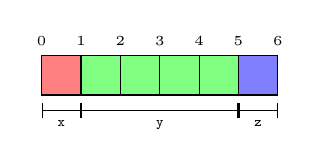
\begin{tikzpicture}
        \draw[fill=red!50] (0,0) rectangle ++(0.5,0.5);
        \draw[fill=green!50] (0.5,0) rectangle ++(2,0.5);
        \draw[fill=blue!50] (2.5,0) rectangle ++(0.5,0.5);
        \draw[thin] (0,0) grid[xstep=0.5cm,ystep=0.5cm] ++(3,0.5);

        \foreach[evaluate={\i*0.5} as \x] \i in {0,...,6} {
          \node[font=\tiny,anchor=south] at (\x,0.5) {\i};
        }

        \begin{scope}[yshift=-2mm]
          \draw[|-|] (0,0) -- ++(0.5,0) node[midway,below,font=\tiny\ttfamily] {x};
          \draw[|-|] (0.5,0) -- ++(2,0) node[midway,below,font=\tiny\ttfamily] {y};
          \draw[|-|] (2.5,0) -- ++(0.5,0) node[midway,below,font=\tiny\ttfamily] {z};
        \end{scope}
      \end{tikzpicture}
    \end{center}

    \onslide<2>
    \begin{center}
      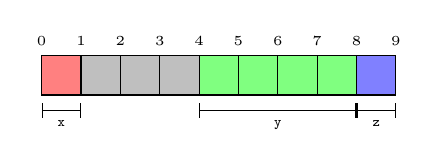
\begin{tikzpicture}
        \draw[fill=gray!50] (0,0) rectangle ++(4.5,0.5);
        \draw[fill=red!50] (0,0) rectangle ++(0.5,0.5);
        \draw[fill=green!50] (2,0) rectangle ++(2,0.5);
        \draw[fill=blue!50] (4,0) rectangle ++(0.5,0.5);
        \draw[thin] (0,0) grid[xstep=0.5cm,ystep=0.5cm] ++(4.5,0.5);

        \foreach[evaluate={\i*0.5} as \x] \i in {0,...,9} {
          \node[font=\tiny,anchor=south] at (\x,0.5) {\i};
        }

        \begin{scope}[yshift=-2mm]
          \draw[|-|] (0,0) -- ++(0.5,0) node[midway,below,font=\tiny\ttfamily] {x};
          \draw[|-|] (2,0) -- ++(2,0) node[midway,below,font=\tiny\ttfamily] {y};
          \draw[|-|] (4,0) -- ++(0.5,0) node[midway,below,font=\tiny\ttfamily] {z};
        \end{scope}
      \end{tikzpicture}
    \end{center}

    \onslide<3>
    \begin{center}
      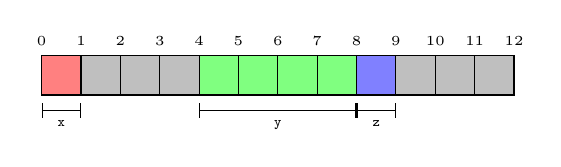
\begin{tikzpicture}
        \draw[fill=gray!50] (0,0) rectangle ++(6,0.5);
        \draw[fill=red!50] (0,0) rectangle ++(0.5,0.5);
        \draw[fill=green!50] (2,0) rectangle ++(2,0.5);
        \draw[fill=blue!50] (4,0) rectangle ++(0.5,0.5);
        \draw[thin] (0,0) grid[xstep=0.5cm,ystep=0.5cm] ++(6,0.5);

        \foreach[evaluate={\i*0.5} as \x] \i in {0,...,12} {
          \node[font=\tiny,anchor=south] at (\x,0.5) {\i};
        }

        \begin{scope}[yshift=-2mm]
          \draw[|-|] (0,0) -- ++(0.5,0) node[midway,below,font=\tiny\ttfamily] {x};
          \draw[|-|] (2,0) -- ++(2,0) node[midway,below,font=\tiny\ttfamily] {y};
          \draw[|-|] (4,0) -- ++(0.5,0) node[midway,below,font=\tiny\ttfamily] {z};
        \end{scope}
      \end{tikzpicture}
    \end{center}
  \end{overprint}
  \begin{overprint}
    \onslide<1>
    \begin{center}
      Unaligned
    \end{center}

    \onslide<2>
    \begin{center}
      Padding added to align members of single object
    \end{center}

    \onslide<3>
    \begin{center}
      Adding padding to make total size a multiple of 4 \\
      This is final memory layout: \texttt{sizeof(Foo) == 12} 
    \end{center}
  \end{overprint}
\end{frame}

\begin{frame}
  \frametitle{Example 2}
  \code[language=c++14,font=\ttfamily\small]{memalign-example2.cpp}
  \begin{overprint}
    \onslide<1>
    \begin{center}
      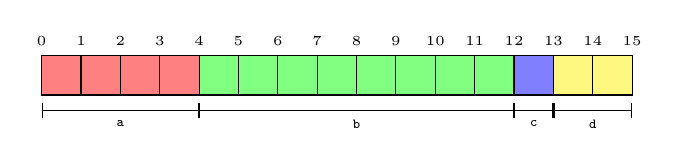
\begin{tikzpicture}
        \draw[fill=red!50] (0,0) rectangle ++(2,0.5);
        \draw[fill=green!50] (2,0) rectangle ++(4,0.5);
        \draw[fill=blue!50] (6,0) rectangle ++(0.5,0.5);
        \draw[fill=yellow!50] (6.5,0) rectangle ++(1,0.5);
        \draw[thin] (0,0) grid[xstep=0.5cm,ystep=0.5cm] ++(7.5,0.5);

        \foreach[evaluate={\i*0.5} as \x] \i in {0,...,15} {
          \node[font=\tiny,anchor=south] at (\x,0.5) {\i};
        }

        \begin{scope}[yshift=-2mm]
          \draw[|-|] (0,0) -- ++(2,0) node[midway,below,font=\tiny\ttfamily] {a};
          \draw[|-|] (2,0) -- ++(4,0) node[midway,below,font=\tiny\ttfamily] {b};
          \draw[|-|] (6,0) -- ++(0.5,0) node[midway,below,font=\tiny\ttfamily] {c};
          \draw[|-|] (6.5,0) -- ++(1,0) node[midway,below,font=\tiny\ttfamily] {d};
        \end{scope}
      \end{tikzpicture}
    \end{center}

    \onslide<2>
    \begin{center}
      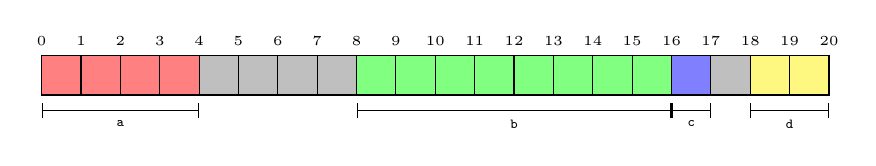
\begin{tikzpicture}
        \draw[fill=gray!50] (0,0) rectangle ++(10,0.5);
        \draw[fill=red!50] (0,0) rectangle ++(2,0.5);
        \draw[fill=green!50] (4,0) rectangle ++(4,0.5);
        \draw[fill=blue!50] (8,0) rectangle ++(0.5,0.5);
        \draw[fill=yellow!50] (9,0) rectangle ++(1,0.5);
        \draw[thin] (0,0) grid[xstep=0.5cm,ystep=0.5cm] ++(10,0.5);

        \foreach[evaluate={\i*0.5} as \x] \i in {0,...,20} {
          \node[font=\tiny,anchor=south] at (\x,0.5) {\i};
        }

        \begin{scope}[yshift=-2mm]
          \draw[|-|] (0,0) -- ++(2,0) node[midway,below,font=\tiny\ttfamily] {a};
          \draw[|-|] (4,0) -- ++(4,0) node[midway,below,font=\tiny\ttfamily] {b};
          \draw[|-|] (8,0) -- ++(0.5,0) node[midway,below,font=\tiny\ttfamily] {c};
          \draw[|-|] (9,0) -- ++(1,0) node[midway,below,font=\tiny\ttfamily] {d};
        \end{scope}
      \end{tikzpicture}
    \end{center}

    \onslide<3>
    \begin{center}
      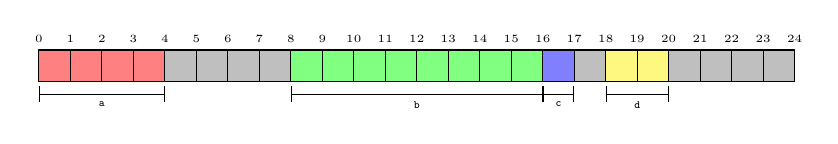
\begin{tikzpicture}[scale=.8,transform shape]
        \draw[fill=gray!50] (0,0) rectangle ++(12,0.5);
        \draw[fill=red!50] (0,0) rectangle ++(2,0.5);
        \draw[fill=green!50] (4,0) rectangle ++(4,0.5);
        \draw[fill=blue!50] (8,0) rectangle ++(0.5,0.5);
        \draw[fill=yellow!50] (9,0) rectangle ++(1,0.5);
        \draw[thin] (0,0) grid[xstep=0.5cm,ystep=0.5cm] ++(12,0.5);

        \foreach[evaluate={\i*0.5} as \x] \i in {0,...,24} {
          \node[font=\tiny,anchor=south] at (\x,0.5) {\i};
        }

        \begin{scope}[yshift=-2mm]
          \draw[|-|] (0,0) -- ++(2,0) node[midway,below,font=\tiny\ttfamily] {a};
          \draw[|-|] (4,0) -- ++(4,0) node[midway,below,font=\tiny\ttfamily] {b};
          \draw[|-|] (8,0) -- ++(0.5,0) node[midway,below,font=\tiny\ttfamily] {c};
          \draw[|-|] (9,0) -- ++(1,0) node[midway,below,font=\tiny\ttfamily] {d};
        \end{scope}
      \end{tikzpicture}
    \end{center}
  \end{overprint}
  \begin{overprint}
    \onslide<1>
    \begin{center}
      Unaligned
    \end{center}

    \onslide<2>
    \begin{center}
      Padding added to align members of single object
    \end{center}

    \onslide<3>
    \begin{center}
      Adding padding to make total size a multiple of 8 \\
      This is final memory layout: \texttt{sizeof(Foo) == 24} 
    \end{center}
  \end{overprint}
\end{frame}


\begin{frame}
  \frametitle{Benchmark: Reading \texttt{uint64\_t}}
  \begin{center}
    \begin{tabular}{cc}
      \textbf{Memory Address} & \textbf{Time} \\
      \toprule
      $8k+0$ & 2189 \\
      $8k+1$ & 3506 \\
      $8k+2$ & 3524 \\
      $8k+3$ & 3611 \\
      $8k+4$ & 3605 \\
      $8k+5$ & 3560 \\
      $8k+6$ & 3566 \\
      $8k+7$ & 3547 \\
    \end{tabular}
  \end{center}
\end{frame}

%%% Local Variables:
%%% mode: latex
%%% TeX-master: "performance"
%%% End:
